\section{openMOS Concept and Technology Stack}
The \gls{openMOS} project developed an open architecture driven by industrial requirements that is able to deliver true system agility without compromising system performance. 
This is viewed as the blueprint for creating easily extendable and adaptable manufacturing operating system, which eases the introduction of new products, work orders and changes in the equipment and allows easy deployment of optimization and changeover management strategies. 
The project builds on plug-and-produce concepts to enable an operating system, while ensuring system performance and resilience, which is critical for dynamic changes which are expected in such systems.

The overall \gls{openMOS} architecture is shown in Figure~\ref{fig:arch}.
Its key elements are \gls{DA}, \gls{MSB}, Agent Cloud and \gls{HMI}.

\gls{DA} wraps the device functionality and offers it as a service, hiding away the low-level process capability (skill) implementation. 
This, in return, allows the lower level orchestrations of composite skill executions, and also provides all necessary interfaces with the higher levels of technology stack, namely \gls{MSB}.
Exposing the skills in a general manner, using a common semantic model allows to seamlessly include new devices and their skills in a production systems, which makes the overall system plug-and-produce capable. 

\gls{MSB} is the central part of the system architecture that allows the vertical as well as horizontal communication across all elements of the technology stack, providing a high degree of flexibility, where the devices can be easily (un)plugged to (from) the system. 
Knowing the underlying system topology, \gls{MSB} is responsible for device discovery, product execution, manages the current state and adjusts the system in case of sudden changes and protocol translation between devices.
It is worth to mention that every communication within an \gls{openMOS} system is done via \gls{MSB}.

The Open Agent-based Manufacturing Operation System Platform (Agent Cloud) is the software layer that collects data from the MSB and persists them in an internal repository, so that external applications can use them to generate statistics and analysis and consequently improve the efficiency of the production system, updating recipes and execution tables crucial for the line execution.

\gls{HMI} is a visual front-end application that runs on a Node.js runtime, it interacts with \gls{MSB} and agent cloud via \gls{SOAP} and \gls{REST} service calls to provide physical line visualization and modification, ramp-up management, as well as products and orders definition and tracking. 

\begin{figure}[tb]
	\centering
	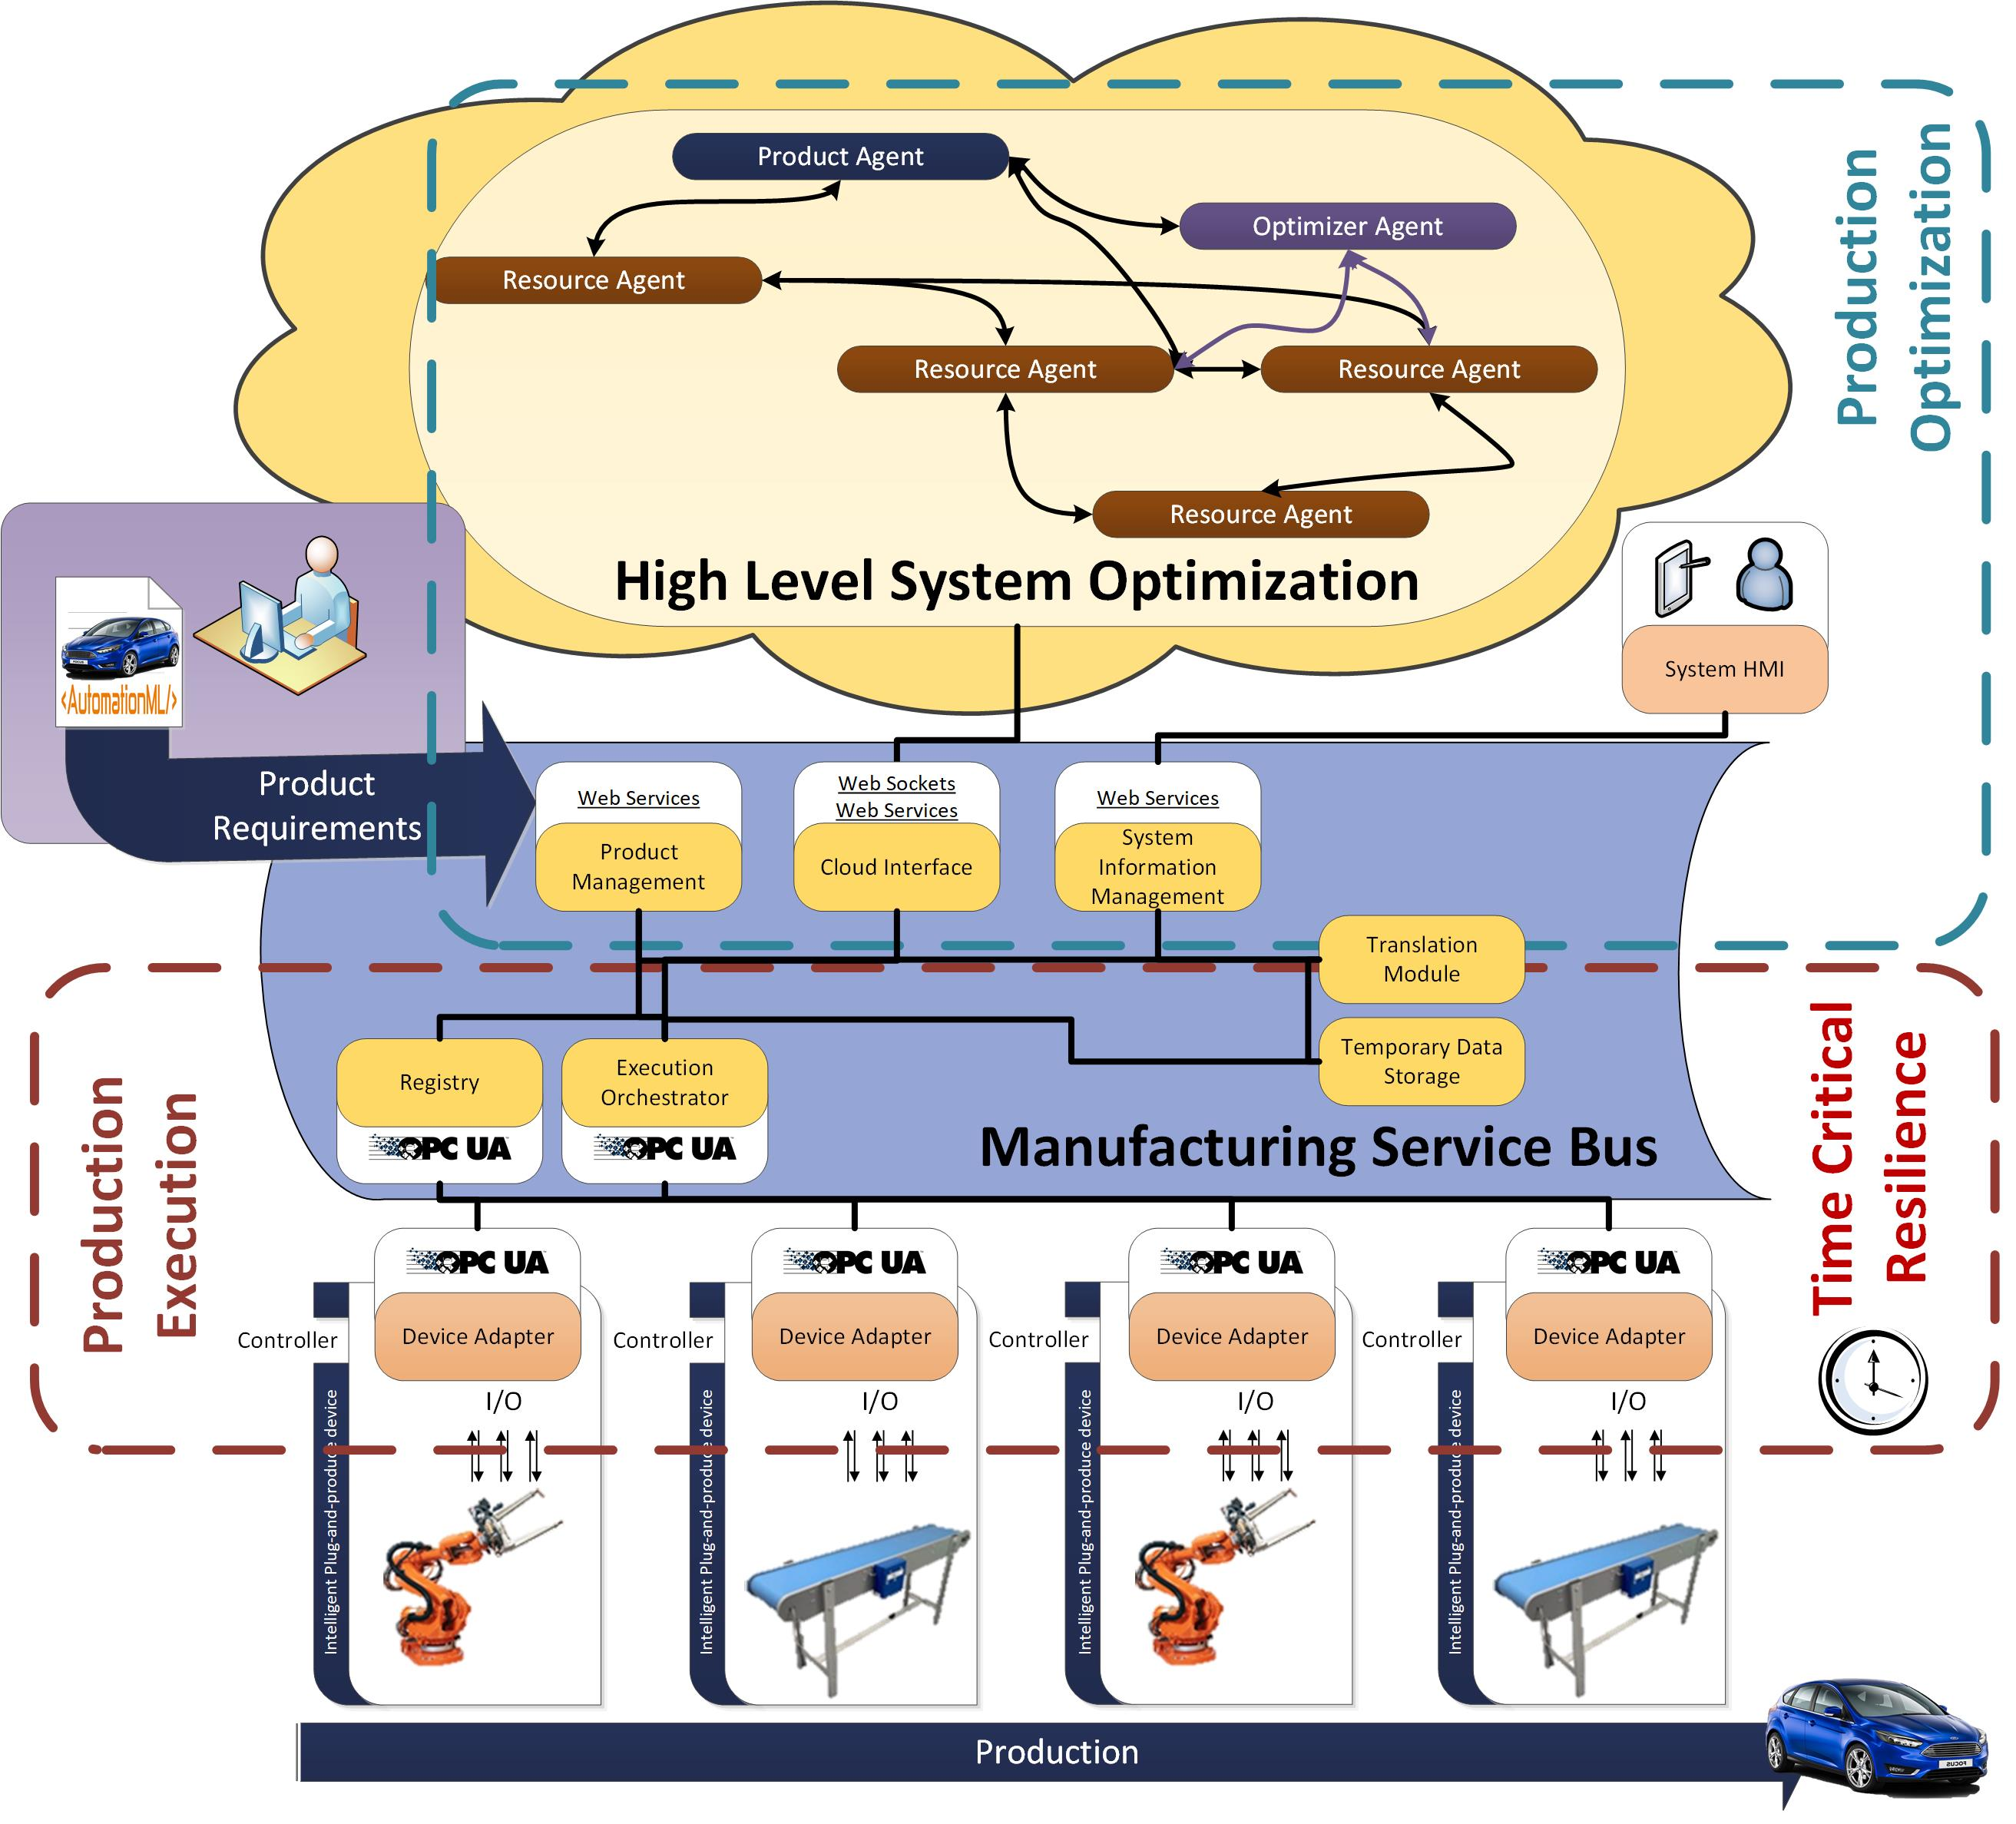
\includegraphics[scale=0.25]{images/diagram}
	\caption{openMOS Architecture}
	\label{fig:arch}
\end{figure}

\subsection{Common Semantic Model}
Each device in the \gls{openMOS} system should contain its self-description that provides all the physical and functional specifications of an equipment module for the creation of a virtual entity, which will be a digital replica of that equipment module. 
In terms of ‘Plug-and-Produce’ devices, they should have embedded information about their process capabilities (skills): the data exchanges and function invocations that constitute a system operation.
\gls{AML} defined in IEC 62714 is used to aggregate all the information of a physical entity (electrical, mechanical, geometry, etc.) in a coherent structure that reflects the overall system hierarchy and can be easily interpreted across multiple engineering domains and tools.
The information stored in the \gls{AML} file can be used to expose the functional capabilities (skills) of the physical entities to its virtual cyber-representations. 
This correlation between the cyber and the physical sides can help the user to virtually design, simulate and evaluate several management strategies.

\subsection{Device Adapter}
The \gls{DA} architecture was developed to support the tasks of device auto-discovery, fast configuration and adaptation, triggering production tasks, reconfiguration (including both hardware and communication reconfiguration) and self-description.
The \gls{DA} implementation uses \textbf{\gls{OPC UA}} as a communication protocol.
The device \textbf{discovery process} is implemented following the \gls{OPC UA} Specification Part 12 that defines \gls{LDS-ME} for this purpose.
This work is released as a contribution to the open source \gls{OPC UA} stacks, \emph{open62541} and \emph{Eclipse Milo}.
The device self-description, being modeled in \gls{AML} is then used to \textbf{automatically generate the \gls{OPC UA} server} information model running on top of a device following the "AutomationML to OPC UA Companion Specification".
The skills, defined in an \gls{AML}, are presented in \gls{OPC UA} namespace as methods, providing a triggering point for \gls{MSB} to execute a production task.
Additionally, the \gls{DA} provides the functionalities to handle the \textbf{(un)plugging of a module, editing recipes and execution tables, making on-the-fly decisions based on the skills outcome, monitoring current execution state, allowing to queue the skill executions}.

\subsection{Manufacturing Service Bus}
The \gls{MSB} is arranged in three major modules: network interface, core and database interface.

The network interface module \textbf{implements all the required protocols} that allow a seamless communication between all \gls{openMOS} modules. 
\gls{MSB} uses \gls{SOAP} services and Web-Sockets for cloud platform data exchange and \gls{OPC UA} for DA communication.

The core module  links together the other modules and represents the core functionalities of the \gls{MSB}, including \textbf{management of the connected devices} (e.g. status, availability, etc.), \textbf{recipe execution orchestrator}, \textbf{data storage} and \textbf{network operation}.

The database interface acts as a proxy that behaves also as a local cache between the openMOS devices and the Agent and Data Cloud platforms, meaning that, all the data collected from the openMOS devices through the MSB is stored locally, temporarily, for redundancy purposes and then sent to the Cloud platform whenever the cloud is online. 
This \textbf{prevents loss of data} and \textbf{ensures the continuous operation} of the system.

\subsection{Agent Cloud and HMI}
From an architectural point of view the agent cloud application consists of three main modules: execution, repository and communication layers.

The execution layer heavily relies on \textbf{\gls{JADE} technology}. 
When \gls{MSB} detects a new \gls{DA} on the network, it alerts the agent cloud platform that deploys a cyberphysical internal abstraction of the device in a form of a \textbf{Java Agent} that holds all the information about the Device Adapter structured according to the openMOS semantic model. 
This agent exists in the cloud until the corresponding \gls{DA} is disconnected from the system and during this time is updating via \gls{MSB} reflecting the real production process.

The repository layer stores the information in a non-relational \textbf{Mongo databas}e to \textbf{track the history} of every change occurring to the system and \textbf{collect the line data}. 

The communication Layer realizes the\textbf{ \gls{SOAP} services} for MSB and optimizers interaction,\textbf{ a Web-socket channel} for MSB-to-agents direct interaction and \textbf{\gls{REST} services} for HMI interaction. 

\gls{HMI} is a Java-script-based application, thus \textbf{\gls{JSON} and \gls{REST} technologies} were selected as the most suitable in this case.